\documentclass[tikz,border=0pt]{standalone}
\usepackage{amsmath,helvet}
\usetikzlibrary{arrows.meta}
\renewcommand{\familydefault}{\sfdefault}
\definecolor{tueblue}{HTML}{0092B5}
\definecolor{muted}{HTML}{646C74}
\begin{document}
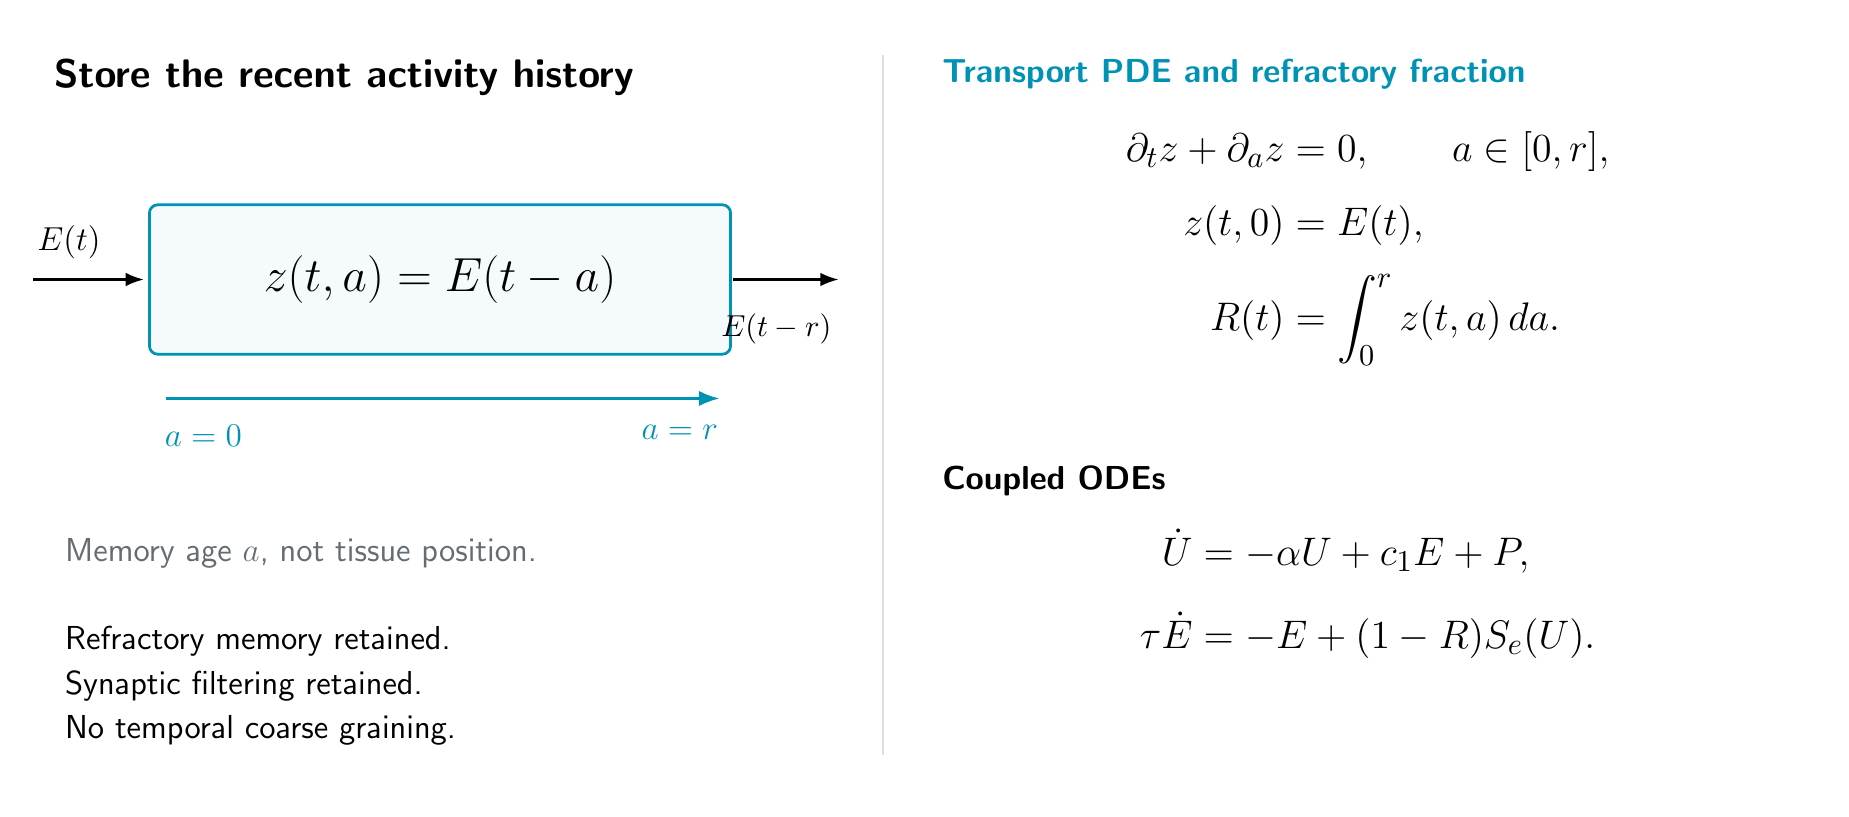
\begin{tikzpicture}[x=1pt,y=1pt,>=Latex]
\path[use as bounding box] (0,0) rectangle (648,275);
\node[anchor=north west,font=\bfseries\fontsize{14}{17}\selectfont] at (6,267)
  {Store the recent activity history};
\draw[rounded corners=3pt,draw=tueblue,fill=tueblue!4,line width=1pt]
  (44,157) rectangle (254,211);
\node[font=\fontsize{17}{20}\selectfont] at (149,184) {$z(t,a)=E(t-a)$};
\draw[->,thick] (2,184)--(42,184);
\node[anchor=south west,font=\fontsize{12}{15}\selectfont] at (0,188) {$E(t)$};
\draw[->,thick] (255,184)--(293,184);
\node[anchor=north east,font=\fontsize{11}{14}\selectfont] at (294,175) {$E(t-r)$};
\draw[->,draw=tueblue,line width=1pt] (50,141)--(250,141);
\node[anchor=north west,text=tueblue,font=\fontsize{12}{15}\selectfont] at (46,135) {$a=0$};
\node[anchor=north east,text=tueblue,font=\fontsize{12}{15}\selectfont] at (253,135) {$a=r$};
\node[anchor=north west,text=muted,font=\fontsize{12}{15}\selectfont] at (10,94)
  {Memory age $a$, not tissue position.};
\node[anchor=north west,font=\fontsize{13}{16}\selectfont,align=left] at (10,62)
  {Refractory memory retained.\\Synaptic filtering retained.\\No temporal coarse graining.};
\draw[gray!25,line width=0.8pt] (309,12)--(309,265);
\node[anchor=north west,text=tueblue,font=\bfseries\fontsize{13}{16}\selectfont] at (327,267)
  {Transport PDE and refractory fraction};
\node[anchor=north west,inner sep=0pt] at (322,242) {\begin{minipage}{324pt}
\fontsize{15}{20}\selectfont
\[
\begin{aligned}
\partial_t z+\partial_a z&=0,\qquad a\in[0,r],\\[4pt]
z(t,0)&=E(t),\\[4pt]
R(t)&=\int_0^r z(t,a)\,da.
\end{aligned}
\]
\end{minipage}};
\node[anchor=north west,font=\bfseries\fontsize{13}{16}\selectfont] at (327,120)
  {Coupled ODEs};
\node[anchor=north west,inner sep=0pt] at (322,96) {\begin{minipage}{324pt}
\fontsize{15}{20}\selectfont
\[
\begin{aligned}
\dot U&=-\alpha U+c_1E+P,\\[7pt]
\tau\dot E&=-E+(1-R)S_e(U).
\end{aligned}
\]
\end{minipage}};
\end{tikzpicture}
\end{document}
